\documentclass[a4paper,twoside]{article}

\usepackage{epsfig}
\usepackage{subfigure}
\usepackage{calc}
\usepackage{amssymb}
\usepackage{amstext}
\usepackage{amsmath}
\usepackage{multicol}
\usepackage{pslatex}
\usepackage{apalike}
\usepackage{fancyhdr}
\usepackage{insticc}
\usepackage[small]{caption}


\begin{document}
\onecolumn \maketitle \normalsize \vfill



%___________________________________________________________________________
\section{\uppercase{Introduction}
\label{sec:introduction}}
%___________________________________________________________________________

\noindent The growing influence of Multi-Agent Systems (MAS) in several fields of research has led
to a significant evolution in its development. On the other hand, the spectacular progress of the
Interactive Graphic Systems (IGS) has contributed to present the information in a more friendly way
using new forms of analysis. The entertainment industry have had a decisive influence on this
progress \cite{Rhyne2000}.

Agents are usually considered to have some generic characteristics that make them difficult to
model \cite{Gilbert2008}. Although there are some common strategies, there is a lack of a unified
design pattern. Hence, some problems arise, such as the difficult reproduction of results
\cite{Axelrod1997}, the lack of a suitable visual representation or the limited capabilities of
interaction.

There are many work environments to develop MASs, but they seldom include advanced visual features.
For instance, in Sociology \cite{Axelrod1997,Gilbert2008}, very specific solutions are used
\cite{Ulicny2001,Reynolds2000}. Netlogo \cite{Wilensky1999} is a useful tool with some basic
graphics to study complex systems.

Some applications of the MASs to Virtual Reality (VR) can also be found. \cite{Maes1995} proposes
an implementation of a virtual world where objects react to gestures of the user. The work of
\cite{Wachsmuth1995} uses the concept of MASs perception applied to VR. In entertainment industry,
agents are usually called bots \cite{Khoo2002} and they are programmed as characters of the game.
These systems are so successful that they are being used in research \cite{Rhyne2000}. An growing
variety of generic development environments are emerging: they implement the most important
features of agents \cite{Gilbert2008}. Repast \cite{North2005} and MASON \cite{Luke2005} are
examples.

As a conclusion, there are a variety of environments, but a model that unifies the definition of
MASs and IGSs has not been proposed. This paper describes our proposal for an integral model based
on grammars to develop complex environments that take advantage of the MASs and the IGSs features.
This system uses a descriptive language and discrete events to specify agents. It will the
interaction with the user and it is independent from the display and the interaction devices. It
could also incorporate a physics engine and the agents could be easily reused.


%___________________________________________________________________________
\section{\uppercase{Proposed Model}
\label{sec:model}}
%___________________________________________________________________________

\noindent In our model, a scene is a set of dynamic and static elements. They are all represented
by a sequence of primitives an transformations of a geometric system $G$. A primitive is not just a
draw primitive but an action on the geometric system that can be visual or not. A transformation is
a modification on the primitives inside its scope of application.

Agents are the dynamic part and they are made of activities and a set of internal states. Each
activity is executed as a reaction to an event. The agents can have a geometrical representation,
defined using primitives and transformations. They also provide different ways of communication.

Formally, each element in the scene is represented by a symbol, which are used to build strings to
describe the scene. The strings follow a language syntax, which is presented as a grammar
\cite{Davis1994} defined by the tuple $M= \ <\Sigma, N, R, s>$, where $\Sigma = P \cup T \cup O
\cup A^D_{ST}$ is the set of terminal symbols ($P$: set of symbols for primitives, $T$: set of
symbols for transformations, $O = \{ \cdotp ( ) \}$: set of symbols of separation and operation,
$A^D_{ST}$: set of symbols for agents with $D$ the set of all possible types of events and $ST$ the
set of possible states), $N$ = \{WORLD, OBJECTS, OBJECT, AGENT, TRANSFORMATION, FIGURE \} is the
set of non-terminal symbols, $s =$ WORLD is the initial symbol and $R$ is the set of grammar rules
defined in the following table.

\begin{table}[h]
\label{tab:rules}
\begin{small}
\begin{center}
\begin{tabular}{|l|}

    \hline

1.\textbf{WORLD} $\rightarrow$ OBJECTS \\

2.\textbf{OBJECTS} $\rightarrow$ OBJECT $|$ OBJECT $\cdot$ OBJECTS \\

3.\textbf{OBJECT} $\rightarrow$ FIGURE $|$ TRANSF. $|$ AGENT \\

4.\textbf{AGENT} $\rightarrow$ $a^d_{st}$ (OBJECTS), $a^d_{st} \in A^D_{ST}, d \in D, st \in ST$ \\

5.\textbf{TRANSFORMATION} $\rightarrow t$ (OBJECTS), $t \in T$ \\

6.\textbf{FIGURE} $\rightarrow$ $p^+$, $p \in P$ \\

    \hline

\end{tabular}
\end{center}
\end{small}
\vspace{-0.3cm}
\end{table}


A string $w \in \Sigma^*$ is generated by $M$, if it can be obtained from the initial symbol using
the given rules. The language $L(M)$ is the set of all the strings which can be generated $L(M) =
\lbrace w \in \Sigma^* \ | \ \text{WORLD} \stackrel{*}{\rightarrow} w \rbrace$. $M$ is a
context-free grammar, so there is a procedure to verify if a scene is correctly described.

Apart from the language syntax, it is necessary to define the semantics. It will be defined with a
denotational method, through mathematical functions.

Rule 6 defines the syntax of a figure as a sequence of primitives. Primitive semantics is defined
by function $\alpha: P \rightarrow G$. Each symbol in $P$ runs a primitive on a geometric system
$G$. So, depending on $\alpha$ and on the geometric system $G$, the result may be different. $G$
represents actions on a specific geometric system (e.g. a graphical library such as OpenGL).

The scope of a transformation is limited by the symbols ``()''. Two functions are used to describe
the semantics of a transformation: $\beta: T \rightarrow G$ (run when the symbol ``('' is
processed), and $\delta: T \rightarrow G$ (run when the symbol ``)'' is found). These two functions
have the same features as $\alpha$, but they are applied to transformations $T$, on the same
geometric system $G$.

Given a string $w \in L(M)$, a new function $\varphi$ is defined to run a sequence of primitives $P$
and transformations $T$ in a geometric system $G$:


\begin{equation}
\begin{small}
    \varphi (w) = \left\{
    \begin{array}{ll}
        \alpha(w) & \mathit{if} \ \ w \in P  \\

        \beta(t); \varphi(v); \delta(t) & \mathit{if} \ \ w = t(v) \wedge v \in L(M) \wedge\\
                                        & \wedge \ t \in T \\

        \varphi(s); \varphi(v)  & \mathit{if} \ \ w = s \cdotp v \wedge s, v \in L(M)
    \end{array}\right\}
\end{small}
\end{equation}



One of the most important features of this system is the independence from a specific graphics
system. The definition of $\alpha$, $\beta$ and $\delta$ provides the differences in behaviour,
encapsulating the implementation details. Therefore, the strings to define a scene may be reused in
other systems.

The semantics of agents is a function which defines its evolution in time. It is called
\textit{evolution function} $\lambda$ and is defined as: $\lambda: L(M) \times E^D \rightarrow
L(M)$, where $E^D$ is the set of events for the device $D$. By applying $\lambda(w, e^{f})$, $w \in
L(M)$ is transformed into another string $u$, which allows the system to evolve. It has a different
expression depending on its evolution, but the general expression is:

\begin{small}
\begin{equation}
    \lambda (a_{st}^{d}(v),e^{f})=
    \left\{
    \begin{array}{ll}
        u \in L(M) & \mathit{if}  \ \ f = d \\
        a_{st}^{d}(v)  & \mathit{if}  \ \ f \neq d
    \end{array}\right\}
\end{equation}
\end{small}

The result $u$ may contain or not the own agent, it can generate other event for the next frame or
change the agent state `$st$'.

The function $\lambda$ defines the \textit{function of the system evolution} $\eta$. Given a set of
events $e^i, e^j, e^k, \dots, e^n$ (denoted as $e^v$, where $v \in D^+$) and a string $w$, it
describes the evolution at a frame. This algorithm uses the operator $\prod_{\forall f \in v}$ to
concatenate strings.

\begin{small}
\begin{equation}
    \eta (w, e^v) = \left\{
    \begin{array}{ll}
        w   & \mathit{if}  \ \ w \in P  \\

        t(\eta (v, e^v))    & \mathit{if}  \ \  w = t(v)  \\

        \underset{\forall f \in v}{ \prod }(\lambda (a_{st}^d (\eta
            (y, e^v)), e^f))    & \mathit{if}  \ \ w = a_{st}^d(y) \\

        \eta (s, e^v) \cdot \eta (t, e^v)   & \mathit{if}  \
\  w = s \cdot t
    \end{array}\right\}
\end{equation}
\end{small}

For the visualization of an agent, it must be first converted into a string of primitives and
transformations. This conversion is done by the \textit{visualization function} $\theta: L(M)
\times E^V \rightarrow L(E)$, where $V \subseteq D$ are events used to create different views,
$E^V$ are events created in the visualization process, and $L(E)$ is the language $L(M)$ without
agents. It is defined as:

\begin{small}
\begin{equation}
    \theta (a_{st}^d(v), e^f) =
    \left\{
    \begin{array}{ll}
        w \in L(E) & \ \ \mathit{if}  \ \ f = d \wedge d \in V \\
        \epsilon  & \ \ \mathit{if}  \ \ f \neq d
    \end{array}\right\}
\end{equation}
\end{small}

As with the function $\lambda$, an algorithm is defined for $\theta$. It returns a string $z \in
L(E)$, given a string $w \in L(M)$ and a set of events $e^v$, where $v \in V^+$ and $V \subseteq
D$. This function is called \textit{function of system visualization} $\pi$ and it is defined as:
$\pi: L(M) \times E^V \rightarrow L(E)$

\begin{small}
\begin{equation}
    \pi (w, e^v) = \left\{
    \begin{array}{ll}
        w   & \mathit{if}  \ \ w \in P^+  \\

        t(\pi (y, e^v))     & \mathit{if}  \ \  w = t(y)  \\

        \underset{\forall f \in v}{ \prod }(\theta (a_{st}^v (\pi
            (y, e^v)), e^f))    & \mathit{if}  \ \ w = a_{st}^v(y) \\

        \pi (s, e^v) \cdot \pi (t, e^v)    & \mathit{if}  \
            \  w = s \cdot t
    \end{array}\right\}
\end{equation}
\end{small}

The activities are run by agents and activated by events under certain conditions. An event is
defined as: {\itshape $e_c^d$ is an event of type $d \in D$ with data $e$, which is carried out
when the condition $c$ is fulfilled.} The condition is omitted if $c = true$. Events may include
information identifying who sent the message. So, it provides a generic communication system that
can implement FIPA or KMQL \cite{Genesereth1995}.

It is necessary to establish the independence between the system and the input devices that
generate events (hardware or software). So, the events needed to make the system respond to the
input devices must be defined. A new function called \textit{event generator} is defined: {\itshape
Let $C^d(t)$ be a function which creates events of type $d$ at the time instant $t$, where $d \in
D$ and $D$ is the set of event types which can be generated. }

It is important to note that event generators encapsulate the device-dependent code.
They also can model the communication processes that exist in a MAS (agent-agent and
agent-environment).

The process which obtains the events produced by the generators is defined as: {\itshape Let $C^*$
be the set of all the event generators which are associated with input devices and $E(C^*, t)$ the
function that collects all the events from all the generators, then:}

\begin{small}
\begin{equation}
\begin{tabular}{l}
    $E(C^*, t) = \left\{
    \begin{array}{ll}
        e(z, C_i(t))   &  \mathit{if}  \ z = E(C^* - C_i, t) \\
        \epsilon   &  \mathit{if} \ C^* = \emptyset
    \end{array}
    \right\}$
    \\
    $e(z, e^i) = \left\{
    \begin{array}{ll}
        z \cdot e^i   &   \mathit{if} \ e^i \notin z \\
        z    &   \mathit{if} \ e^i \in z
    \end{array}
    \right\}$
\end{tabular}
\end{equation}
\end{small}

Once all the elements involved in the model have been defined, the algorithm which carries out the
entire system can be established:

\begin{center}
\begin{small}
\begin{tabular}{|ll|}
    \hline
    1. & $w = w_o$; $t = 0$ \\
    2. & $e^* = E(G^*, t)$ \\
    3. & $e^v =$ events of $e^*$ where $v \in V^+$ \\
    4. & $e^u = e^* - e^v$ \\
    5. & $w_{next} = \eta(w, e^u)$ \\
    6. & $v =  \pi(w, e^v)$ \\
    7. & $g = \varphi(v)$ \\
    8. & $w = w_{next}; \ \ t = t + 1$ \\
    9. & If $w = \epsilon$ then go to 11 \\
    10. & Go to 2 \\
    11. & End \\
\hline
\end{tabular}
\end{small}
\end{center}

\noindent where $w_o$ is the intial string, $e^*$ are the events generated at a frame $t$, $G^*$ =
\{All the event generators\}, $D$ = \{All the possible events\}, $V$ = \{All the visual events\};
$V \subseteq D$, $e^v$ all the visual events, $e^u$ all the non-visual events and $g$ the output
device.

Steps 2, 3 and 4 manage the system events. In step 5, the evolution algorithm is called to obtain
the string for the next frame. In steps 6 and 7, the visualization of the system is performed. In
step 8, the next iteration is prepared. The algorithm finishes if the following string is empty.

%___________________________________________________________________________
\section{\uppercase{Case of Study}
\label{sec:case_study}}
%___________________________________________________________________________

\noindent This example is an application to simulate fires in forests caused by lightning
\cite{John2007}. The system consists of an agent to define the forest that can create other agents:
trees (with a given probability $g$) and lightning (with a probability $f$). If lightning are
created in the same position as a tree, it will burn as well as the trees around it (Figure
\ref{fig:example1}).

\begin{figure}[htb]
    \centering
    \begin{tabular}{cc}
        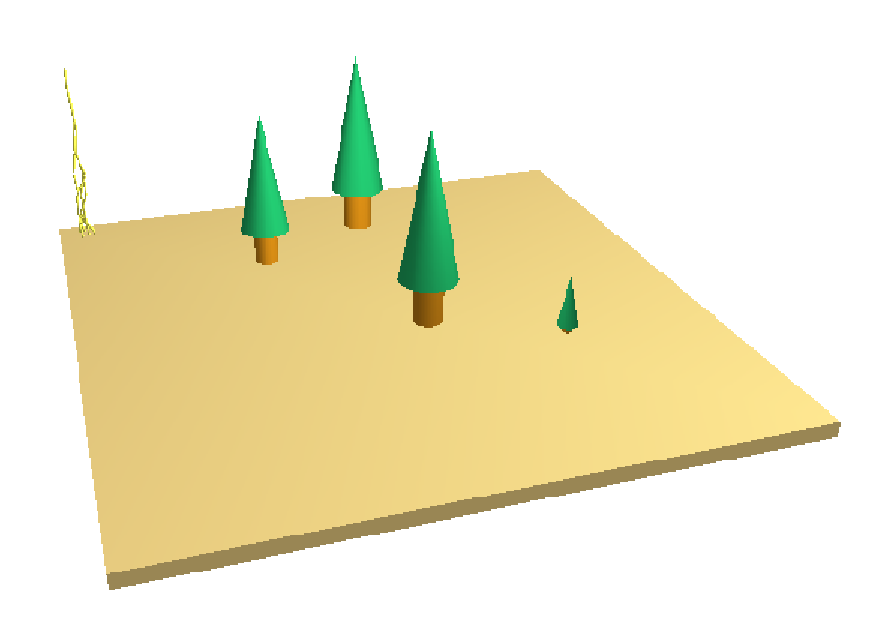
\includegraphics[width=3.5cm]{figureEx1} &
        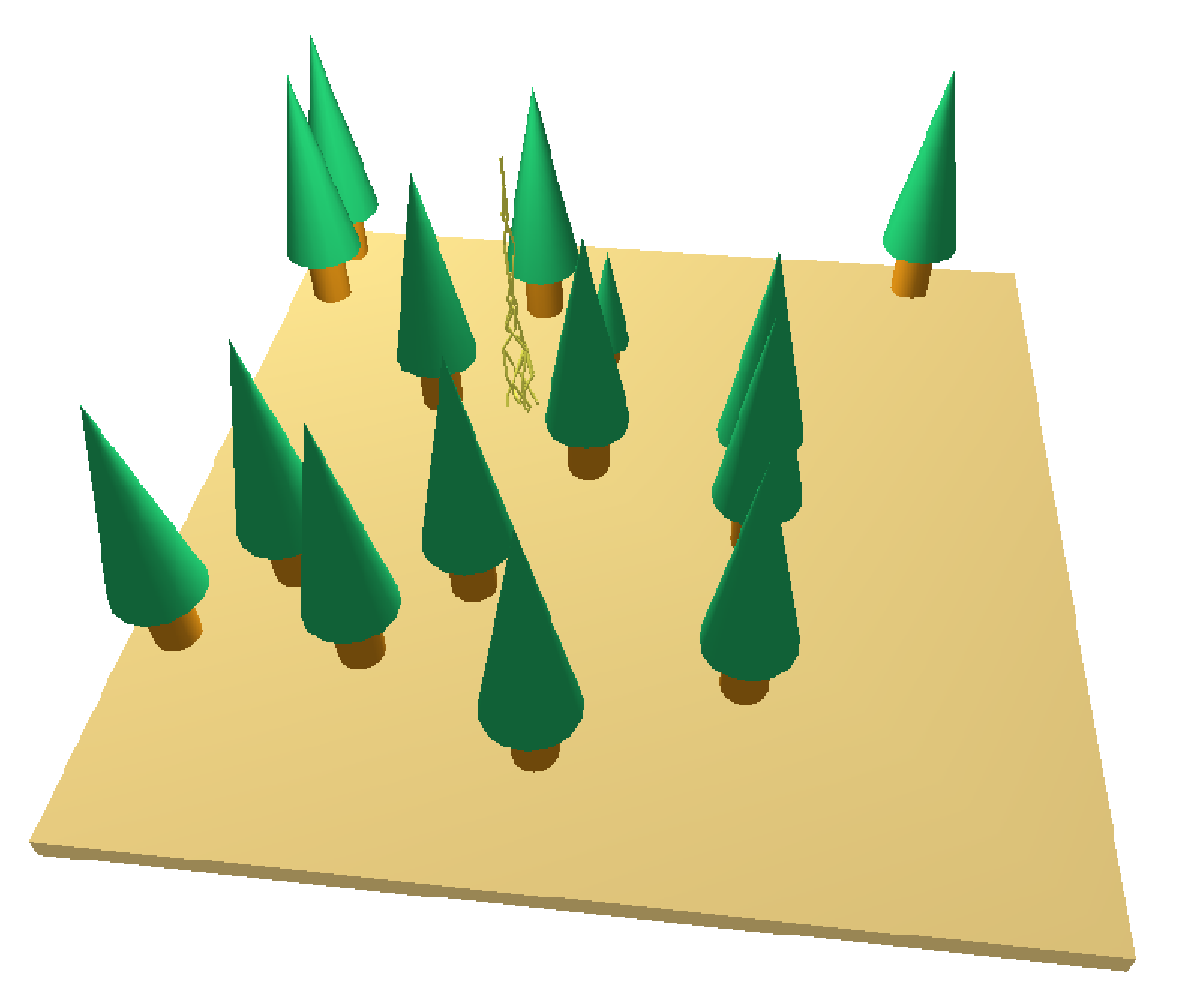
\includegraphics[width=3.5cm]{figureEx2}
    \end{tabular}
    \caption{\label{fig:example1} Examples of different simulation states}
\end{figure}


To model this example, four elements are defined:
events, event generators, agents and primitives.

Events are used to produce the necessary activity of system.
The events defined for this example are:

%\vspace{-0.4cm}

\begin{table}[h]
\begin{center}
\begin{small}
    \begin{tabular}{|l|l|}
        \hline $t$   & Event generated to increase the time.\\
        \hline $c$   & Creates a tree at the position $(i, j)$ of the forest.\\
        \hline $f$   & Creates a bolt of lightning at position $(i, j)$.\\
        \hline $e$   & Eliminates the tree of the position $(i, j)$.\\
        \hline $b$   & Burns the tree at position $(i, j)$.\\
        \hline $v$   & Draws using a graphics library (e.g. OpenGL).\\
        \hline
\end{tabular}
\end{small}
\end{center}
\vspace{-0.3cm}
\end{table}


%\vspace{-1.5cm}

\noindent The next step is to define the event generators:

%\vspace{-0.4cm}

\begin{table}[h]
\begin{center}
\begin{small}
    \begin{tabular}{|l|l|}
        \hline ($C_{time}$)   & Generate an event $e^t$ at instant $t$\\
        \hline ($C_{forest}$)   & Create tree ($e^{c}$) or lightning ($e^{f}$)\\
        \hline ($C_{draw}$)   & Generate draw event\\
        \hline
\end{tabular}
\end{small}
\end{center}
\vspace{-0.3cm}
\end{table}


%\vspace{-1.5cm}


The following table shows the primitives and the transformations that make up the scene. The
functions ${\alpha}$, ${\beta}$ and ${\delta}$ define them.

%\vspace{-0.4cm}

\begin{table}[h]
\begin{center}
\begin{small}
    \begin{tabular}{|l|l|}
        \hline \itshape Primitive & \itshape Description\\
        \hline $TR$   & Draw a tree\\
        \hline $TR_b$ & Draw a burning tree\\
        \hline $FA$   & Draw a bolt of lightning\\
        \hline $BO$   & Draw a grid of NxN \\
        \hline
        \hline \itshape Transformations & \itshape Description\\
        \hline $D_{(i,j)}$ & Translate (i,j)\\
        \hline $S_{(s)}$ & Scale (n) units\\
        \hline
    \end{tabular}
\end{small}
\end{center}
\vspace{-0.3cm}
\end{table}


%\vspace{-1.5cm}
The evolution function $\lambda$ and the graphical representation $\pi$ are presented next. The
agent defined for trees ($TR$) has three internal states $st = \{s1, s2, s3 \}$: $s1$ growth, $s2$
adult tree and $s3$ burning tree. This is an example of different representation for an agent
depending on its internal state. The function $Nbo$ sends burn events $e^b$ to all the neighbour
trees, creating a chain reaction (agent-agent communication). An example of agent-environment
communication is made between the forest and the generator $C_{forest}$.


\begin{table}[h]
\begin{center}
\begin{small}
\begin{tabular}{|p{0.11\linewidth}|p{0.75\linewidth}|}

    \hline
    \itshape Agent &
    \itshape Function ${\lambda}$ and ${\pi}$\\

    \hline
    \itshape BO Forest &
    \begin{tabular}{l}
        $\lambda(BO^{cfe}, e^{i}) = $ \\
        $\left\{
        \begin{array}{ll}
            TR_{s1}^{t=1} \cdot BO^{cfv}    & \ \ \ i = c \\
            FA^{t=1}   \cdot BO^{cfv}   & \ \ \ i = f \\
            BO^{cfe}            & \ \ \ i = e \\
            BO^{cfe}            & \ \ \ i \neq c,f,e
        \end{array}
        \right\}$ \\
        \\
        $\pi (BO^{v}, e^{i}) = $\\
        $\left\{
        \begin{array}{ll}
            BO          & \ \ \   i = v \\
            \epsilon    & \ \ \   i \neq v
        \end{array}
        \right\}$
    \end{tabular}   \\

    \hline
    \itshape TR Tree &
    \begin{tabular}{l}
        $\lambda(TR_{st}^x, e^{i}) = $\\
        $\left\{
        \begin{array}{ll}
            TR_{s1}^{t+1}       & i = t \wedge t+1 \leqslant N \wedge s = s1 \\
            TR_{s2}^{b}         & i = t \wedge t+1 > N \wedge s = s1 \\
            TR_{s3}^{t=1} \wedge & \\
            \ \ \wedge \Delta Nbo^{b}         & i = b > N \wedge s = s2 \\
            TR_{s3}^{t+1}       & i = t \wedge s = s3 \\
            \Delta e^{e}        & i = t \wedge  t+1 > N  \wedge s = s3 \\
            TR_{st}^{t}         & i \neq t \wedge   i \neq b \\
        \end{array}
        \right\}$ \\
        \\
        $\pi (TR_{st}^{v}, e^{i}) = $\\
        $\left\{
        \begin{array}{ll}
            D_{(i, j)}( S_{(n)} (TR) )    & \ \ \   i = v \wedge st = s1 \\
            D_{(i, j)}( TR )        & \ \ \   i = v \wedge st = s2 \\
            D_{(i, j)}( S_{(-n)} (TR) )   & \ \ \   i = v \wedge st = s3 \\
            \epsilon            & \ \ \   i \neq v
        \end{array}\right\}$
    \end{tabular}   \\


    \hline
    \itshape FA Lightning &
    \begin{tabular}{lll}
        $\lambda (FA^{t}, e^{i}) = $\\
        $\left\{
        \begin{array}{ll}
            FA^{t+1}        & \ \ \  i = t \wedge t+1 \leqslant N \\
            \Delta e^{b}        & \ \ \  i = t \wedge t+1 > N \\
            FA^{t}          & \ \ \  i \neq t
        \end{array}
        \right\}$ \\
        \\
        $\pi (FA^{v}, e^{i}) = $\\
        $\left\{
        \begin{array}{ll}
            D_{(i, j)}(FA)          & \ \ \   i = v \\
            \epsilon            & \ \ \   i \neq v
        \end{array}
        \right\}$
    \end{tabular}   \\

    \hline
\end{tabular}
\end{small}
\end{center}
\vspace{-0.3cm}
\end{table}






%\vspace{-1cm}


%___________________________________________________________________________
\section{\uppercase{Conclusions}
\label{sec:conclusions}}
%___________________________________________________________________________

\noindent In this paper a proposal to unify the most relevant features of MASs and IGSs has been
presented. The proposed model uses a context-free language to define the elements. Although further
work needs to be done, the use of a descriptive language seems to have several advantages.
Firstly, the definition of the scene is reusable and independent from the platform.
The use of event generators also makes the interaction with the user
independent from the hardware. 
Event generators are also used to implement the communication,
both agent-agent and agent-environment.

As future work the model will be applied to other problems to validate its
features. New possibilities such as probabilistic learning strategies or genetic algorithms will
be considered.



%___________________________________________________________________________

%___________________________________________________________________________



\renewcommand{\baselinestretch}{0.98}
\bibliographystyle{apalike}
{\small

\begin{thebibliography}{14}

\bibitem[Axelrod, 1997]{Axelrod1997}
R. Axelrod (1997).
Advancing the Art of Simulation in the Social Sciences.
\emph{Simulating Social Phenomena}, Springer.

\bibitem[Genesereth, 1995]{Genesereth1995}
Michael R. Genesereth, Steven P. Ketchpel (1995).
\newblock Software Agents.
\newblock \emph{Communications of the ACM}.

\bibitem[Gilbert, 2008]{Gilbert2008}
N. Gilbert (2008).
\newblock Agent-Based Models.
\newblock \emph{SAGE Publications}.

\bibitem[Miller, 2007]{John2007}
John H. Miller (2007).
\newblock Complex Adaptative Systems.
\newblock \emph{Princeton University Press}.

\bibitem[Khoo, 2002]{Khoo2002}
Aaron Khoo, Robert Zubek (2002).
\newblock Applying Inexpensive AI Techniques to Computer Games.
\newblock \emph{IEEE Intelligent Systems} July-August.

\bibitem[Luke, 2005]{Luke2005}
Sean Luke, Claudio Cioffi-Revilla, Liviu Panait, and Keith Sullivan (2005).
\newblock MASON: A New Multi-Agent Simulation Toolkit.
\newblock \emph{Vol. 81, SAGE Journals}.

\bibitem[Maes, 1997]{Maes1995}
P. Maes, T. Darrell, B. Blumberg, A. Pentland (1997).
\newblock The ALIVE System:Wireless, Full-body Interaction with Autonomous Agents.
\newblock \emph{ACM Multimedia Systems, Vol.5, No.2, pp.105-112}.

\bibitem[North, 2005]{North2005}
M.J. North, T.R. Howe, N.T. Collier, J.R. Vos (2005).
\newblock The Repast Simphony Runtime System.
\newblock \emph{Generative Social Processes, Models, and Mechanisms}.

\bibitem[Reynolds, 2000]{Reynolds2000}
Craig Reynolds (2000).
\newblock Interaction with Groups of Autonomous Characters.
\newblock \emph{Game Developers Conference}.

\bibitem[Rhyne, 2000]{Rhyne2000}
Theresa-Marie Rhyne (2000).
\newblock Computer Games’Influence on Scientific and Information Visualization.
\newblock \emph{Entertainment Computing}.

\bibitem[Ulicny, 2001]{Ulicny2001}
B. Ulicny, D. Thalmann (2001).
\newblock Crowd simulation for interactive virtual environments and VR training systems.
\newblock \emph{Computer Animation and Simulation, Springer}.

\bibitem[Wilensky, 1999]{Wilensky1999}
Wilensky, U. (1999).
\newblock NetLogo. User Manual.

\bibitem[Wachsmuth, 1995]{Wachsmuth1995}
Ipke Wachsmuth, Yong Cao (1995).
\newblock Interactive Graphics Design with Situated Agents.
\newblock \emph{Graphics and Robotics}.

\bibitem[Martin, 1994]{Davis1994}
D.Martin, R.Sigal, E.J.Weyuker (1994).
\emph{Computability, Complexity, and Languages, Fundamentals of Theoretical Computer Science},
2nd~ed, Elsevier Science.

\end{thebibliography}

}
\renewcommand{\baselinestretch}{1}




%___________________________________________________________________________


% PARA AJUSTAR LA ULTIMA PAGINA Y QUE LAS DOS COLUMNAS QUEDEN IGUALADAS
%\vfill
%\enlargethispage{-cm}




\end{document}
